
\documentclass[10pt,conference]{IEEEtran}

% ---------- Packages ----------
\usepackage[utf8]{inputenc}
\usepackage[T1]{fontenc}
\usepackage{times}
\usepackage{amsmath, amssymb}
\usepackage{graphicx}
\usepackage{booktabs}
\usepackage{multirow}
\usepackage{array}
\usepackage{url}
\usepackage{xcolor}
\usepackage{hyperref}
\usepackage{enumitem}
\usepackage{float}

% ---------- Hyperref ----------
\hypersetup{
    colorlinks=true,
    linkcolor=blue,
    filecolor=blue,
    urlcolor=blue,
    citecolor=blue
}

% ---------- Helper commands ----------
\newcommand{\todo}[1]{\textcolor{red}{[TODO: #1]}}
\newcommand{\best}[1]{\textbf{#1}}

\title{Learning Visuomotor Policies for Cabinet Manipulation:\\
Representation, Data Regime, and Policy Class}

\author{
\IEEEauthorblockN{Satyajit Kumar \and Noah Cylich}
}

\begin{document}

\maketitle

\begin{abstract}
We study the \textit{OpenCabinet} manipulation task in RoboCasa, where a robot must locate a cabinet, reach the handle, and open the door across randomized kitchen layouts. Our project investigates how observation representation, model class, and dataset size affect imitation learning performance in this setting. We began with low-dimensional state-only policies, then explored frozen visuomotor encoders, oracle door-position features, handle-relative state features, and head-to-head comparisons between behavioral cloning (BC) and diffusion policies. Our experiments show that state-only policies fail because they lack object information, and that the first major improvement comes from oracle geometric features. The key breakthrough, however, is shifting from door-centric to handle-centric representations, which align the policy with the true manipulation target. In the original 107-demo regime, our best model is a BC U-Net with handle-relative features, achieving \best{44\% success over 100 evaluation episodes}. After scaling to a combined 607-demo dataset, a diffusion U-Net surpasses BC and reaches \best{49\% success}. Overall, our results show that representation matters more than architecture early on, while diffusion becomes advantageous only after sufficient data scaling.
\end{abstract}

\section{Introduction}
Robotic manipulation in realistic environments requires policies that can perceive task-relevant objects, plan temporally consistent actions, and execute contact-rich behaviors robustly. Cabinet opening is a representative example of this challenge: the robot must not only move toward a cabinet, but also target the handle, align its end effector, and pull the door open under varying scene layouts.

In this project, we study the RoboCasa \textit{OpenCabinet} task through the lens of imitation learning. Rather than asking only which policy architecture works best, we focus on three broader questions: what information the policy must observe to solve the task, how behavioral cloning and diffusion policies compare in the low-data regime, and at what point additional data changes which method is most effective.

Our final conclusion is that the largest early gains come from \emph{representation design}, not architecture alone. State-only policies fail because they cannot localize the cabinet. Door-centric oracle features help, but the decisive improvement comes from handle-relative representations. Once those are in place, BC is the best method in the 107-demo regime, while diffusion overtakes BC only after scaling the dataset substantially.

\begin{figure}[!t]
\centering
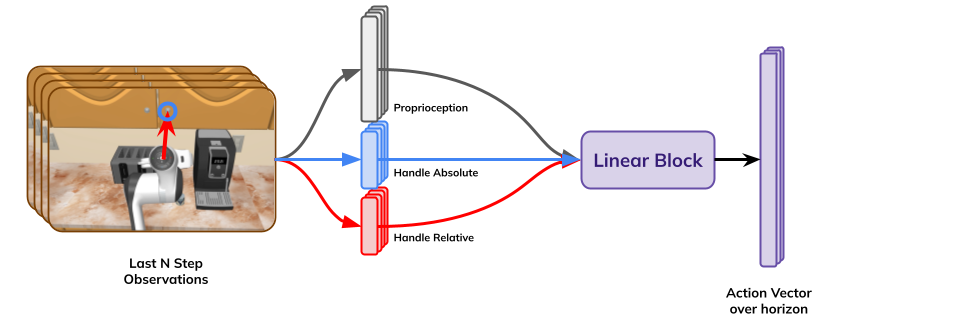
\includegraphics[width=\columnwidth]{assets/BC_arch.png}\\[-0.3em]
{\footnotesize (a) BC U-Net architecture.\par}
\vspace{0.4em}
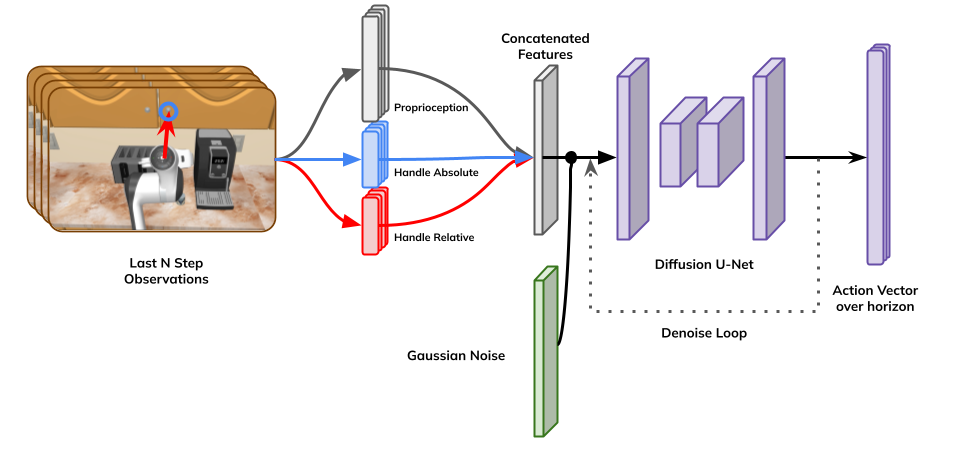
\includegraphics[width=\columnwidth]{assets/Diffusion_arch.png}\\[-0.3em]
{\footnotesize (b) Diffusion U-Net architecture.\par}
\caption{Architecture diagrams for the two final policy families. BC directly predicts an action chunk from observation context, while diffusion iteratively denoises a noisy action chunk conditioned on the same context.}
\label{fig:policy-architectures}
\end{figure}

\section{Problem Statement}
The goal of this project is to train a policy that opens a kitchen cabinet door in the RoboCasa \textit{OpenCabinet} task using imitation learning from demonstrations.

\subsection{Task}
Each evaluation episode spawns a randomized kitchen from a large set of possible layouts. A successful rollout requires the robot to identify the cabinet location, approach the correct handle, establish appropriate contact or grasp, and pull the cabinet door open within the episode horizon.

\subsection{Inputs and Outputs}
The dataset provides a 16-dimensional proprioceptive state, RGB observations from multiple cameras, and 12-dimensional demonstration actions. Across the project, we also experiment with additional oracle state features derived from simulation replay, including door position, handle position, relative geometry, and hinge angle. The policy outputs action sequences controlling end-effector motion, gripper behavior, and other robot controls.

\subsection{Evaluation Metrics}
We evaluate models using three main criteria: success rate, defined as the fraction of rollouts that open the cabinet sufficiently; distance reduction, measuring how much the robot reduces its distance to the target (door or handle); and qualitative rollout behavior, including approach quality, near-misses, and failure modes.

\section{Method Overview}
Our project proceeded as a sequence of increasingly targeted experiments. Instead of fixing one architecture and tuning it, we used the task to diagnose what information and modeling choices were actually necessary.

\subsection{Phase 1: State-Only Diffusion Policies}
We first implemented diffusion policies using only the raw 16-dimensional proprioceptive state. We trained multiple denoising backbones, including MLP, 1D U-Net, and Transformer architectures. These models fit the demonstration actions on the training set, confirming that the diffusion pipeline worked technically, but all achieved \best{0\% success} at evaluation. This established that the core problem was \emph{missing task information}: the state did not contain cabinet location.

\subsection{Phase 2: Visuomotor Models}
We next explored image-conditioned policies using frozen visual encoders. These included ImageNet ResNet-18 with global average pooling, ImageNet ResNet-18 with spatial softmax, R3M-based features, and a published-style diffusion-policy visual configuration. While these models improved approach behavior, especially when spatial structure was preserved, they still failed to solve the full task at our data scale.

\subsection{Phase 3: Oracle Door Features}
To separate perception from control, we augmented the observation with oracle door geometry extracted from simulator replay. This produced the first task success and showed that once object location is provided, the policy can begin to approach and interact more meaningfully with the cabinet.

\subsection{Phase 4: BC vs. Diffusion Under Shared Features}
After confirming that geometry was the main bottleneck, we compared direct behavioral cloning (BC) against diffusion policies under shared experimental settings. We evaluated MLP, Transformer, and U-Net backbones for both BC and diffusion, along with multiple training horizons and validation-based early stopping. This revealed a key low-data result: in the 107-demo regime, small BC models often outperformed diffusion in task performance while training significantly faster.

\subsection{Phase 5: Handle-Relative State Design}
The biggest conceptual change in the project was recognizing that targeting the door centroid is not equivalent to targeting the handle. We therefore replayed demonstrations in MuJoCo to extract handle-site positions and constructed handle-relative features such as handle position, handle-to-end-effector displacement, and hinge angle. These representations aligned the observation with the true physical target of the task and produced a major increase in success.

\subsection{Phase 6: Data Scaling}
Finally, we expanded from the original 107-demo dataset to a combined 607-demo dataset and repeated the best BC and diffusion experiments. This allowed us to test whether diffusion had fundamentally failed or had simply been starved of data.

\section{System Design and Implementation}
\subsection{Policy Classes}
We implemented and compared two policy families:

\textbf{Behavioral Cloning (BC):} A direct supervised mapping from observations (or observation histories) to actions / action chunks.

\textbf{Diffusion Policy:} An iterative denoising model that predicts actions through a diffusion process. We implemented DDPM/DDIM-style training and inference along with multiple denoising backbones.

\subsection{Backbones}
Across both BC and diffusion settings, we evaluated MLP, 1D U-Net, and Transformer backbones to understand how architecture interacts with representation and data regime.

\subsection{Temporal Action Modeling}
We experimented with action chunking and temporal context. In the strongest low-data models, temporal coherence proved important: purely reactive one-step policies were much less effective than chunked-action models with short history.

\subsection{Feature Engineering}
A large portion of the project focused on observation design. We explored a range of features, including raw proprioception, door position and orientation, global end-effector pose, door-to-end-effector relative geometry, scalar distance features, handle position, handle-to-end-effector displacement, and hinge angle. These experiments were critical in identifying which representations aligned best with the manipulation objective.

\subsection{Infrastructure and Debugging}
We also implemented substantial supporting infrastructure, including cached preprocessing of oracle state features, handle-position extraction via simulator replay, parallel evaluation workers for faster rollout statistics, corrected action-mapping and gripper-threshold logic, and validation-based early stopping to avoid severe overfitting.

The core diffusion-policy implementation lives in the \texttt{cabinet\_door\_project/diffusion\_policy/} package, which contains configuration, data loading, schedulers, training, inference, evaluation utilities, and the MLP / U-Net / Transformer backbones. Experiment-specific scripts include \texttt{compare\_bc\_vs\_diffusion.py} for matched BC-versus-diffusion studies, \texttt{ablation\_sweep.py} for large feature and method sweeps, \texttt{preprocess\_all\_states.py} and \texttt{generate\_door\_positions.py} for oracle replay preprocessing, \texttt{bc\_handle.py} for the handle-aware BC pipeline, and \texttt{validate\_best.py} for 100-episode validation of the strongest pretrain-only BC U-Net.

\section{Experimental Setup}
\subsection{Dataset}
The original dataset contains \best{107 demonstrations} and \best{37,492 timesteps} across randomized kitchen layouts, with 16-dimensional proprioceptive states and 12-dimensional actions. We later downloaded the target split and expanded to a combined dataset of \best{607 demonstrations} and \best{221,516 frames}.

\subsection{Hardware}
All main experiments were run on an \best{NVIDIA A100 80GB VM on GCP}. Later evaluation was performed on a 12-core workstation using parallel rollout workers, where we found that four workers provided the best throughput before CPU contention dominated.

\subsection{Evaluation Protocol}
All rollout evaluations used a 500-step horizon. During rapid iteration we often used 16 or 20 episodes, but the main headline pretrain-only result was validated over 100 episodes. In the main validation scripts, we used a relaxed one-door-open success criterion: a rollout counts as successful once at least one cabinet hinge angle exceeds 0.3 rad. The final project-page summary reports the 44\% and 49\% headline numbers under this same one-door-open framing.

Our best pretrain-only model was a BC U-Net using handle-aware features. After retraining and evaluating over 100 episodes under the one-door-open hinge-angle criterion, it achieved \best{44\% success (44/100)}, representing the strongest low-data performance in the project and a clear improvement over earlier handle-aware transformer baselines.

\section{Results}
\subsection{Stage 1: State-Only and Early Visuomotor Results}
Our earliest experiments showed that raw proprioception alone is insufficient. Even when diffusion models fit the training data well, they achieved no meaningful task success because they lacked any information about cabinet location.

Frozen visuomotor encoders improved approach behavior modestly, especially when spatial structure was preserved. In particular, spatially aware pooling outperformed global average pooling, suggesting that preserving \emph{where} visual features occur matters for manipulation. However, these models still did not solve the full task reliably at our data scale. Taken together, these early results indicate that the main bottleneck was missing task information rather than action-model capacity alone.

\subsection{Stage 2: Oracle Door Features}
Adding oracle door geometry produced the first successful rollouts and provided the clearest early evidence that explicit object-location information helps.

However, these models still targeted the door body rather than the handle, which limited success. They often approached the cabinet but stopped short of an effective grasp-and-pull interaction. This isolated the remaining difficulty: once cabinet location is known, the task is no longer coarse localization but precise interaction at the true grasp point.

\begin{table}[H]
\centering
\caption{Oracle door feature results.}
\footnotesize
\setlength{\tabcolsep}{3pt}
\begin{tabular}{@{}>{\raggedright\arraybackslash}p{0.18\columnwidth}>{\raggedright\arraybackslash}p{0.29\columnwidth}c>{\raggedright\arraybackslash}p{0.31\columnwidth}@{}}
\toprule
Model & Features & Success & Notes \\
\midrule
Diffusion U-Net & Door position & 5\% & First success (1/20), $\sim$38\% distance reduction \\
BC MLP & Door position + door-to-EEF + scalar distance & 0\% & 51\% distance reduction, but no successful opening \\
BC MLP / BC MLP + dropout & Strongest door-centric oracle features & 0\% & Door-centric methods plateaued at 55\% distance reduction \\
\bottomrule
\end{tabular}
\end{table}

\begin{figure}[t]
\centering
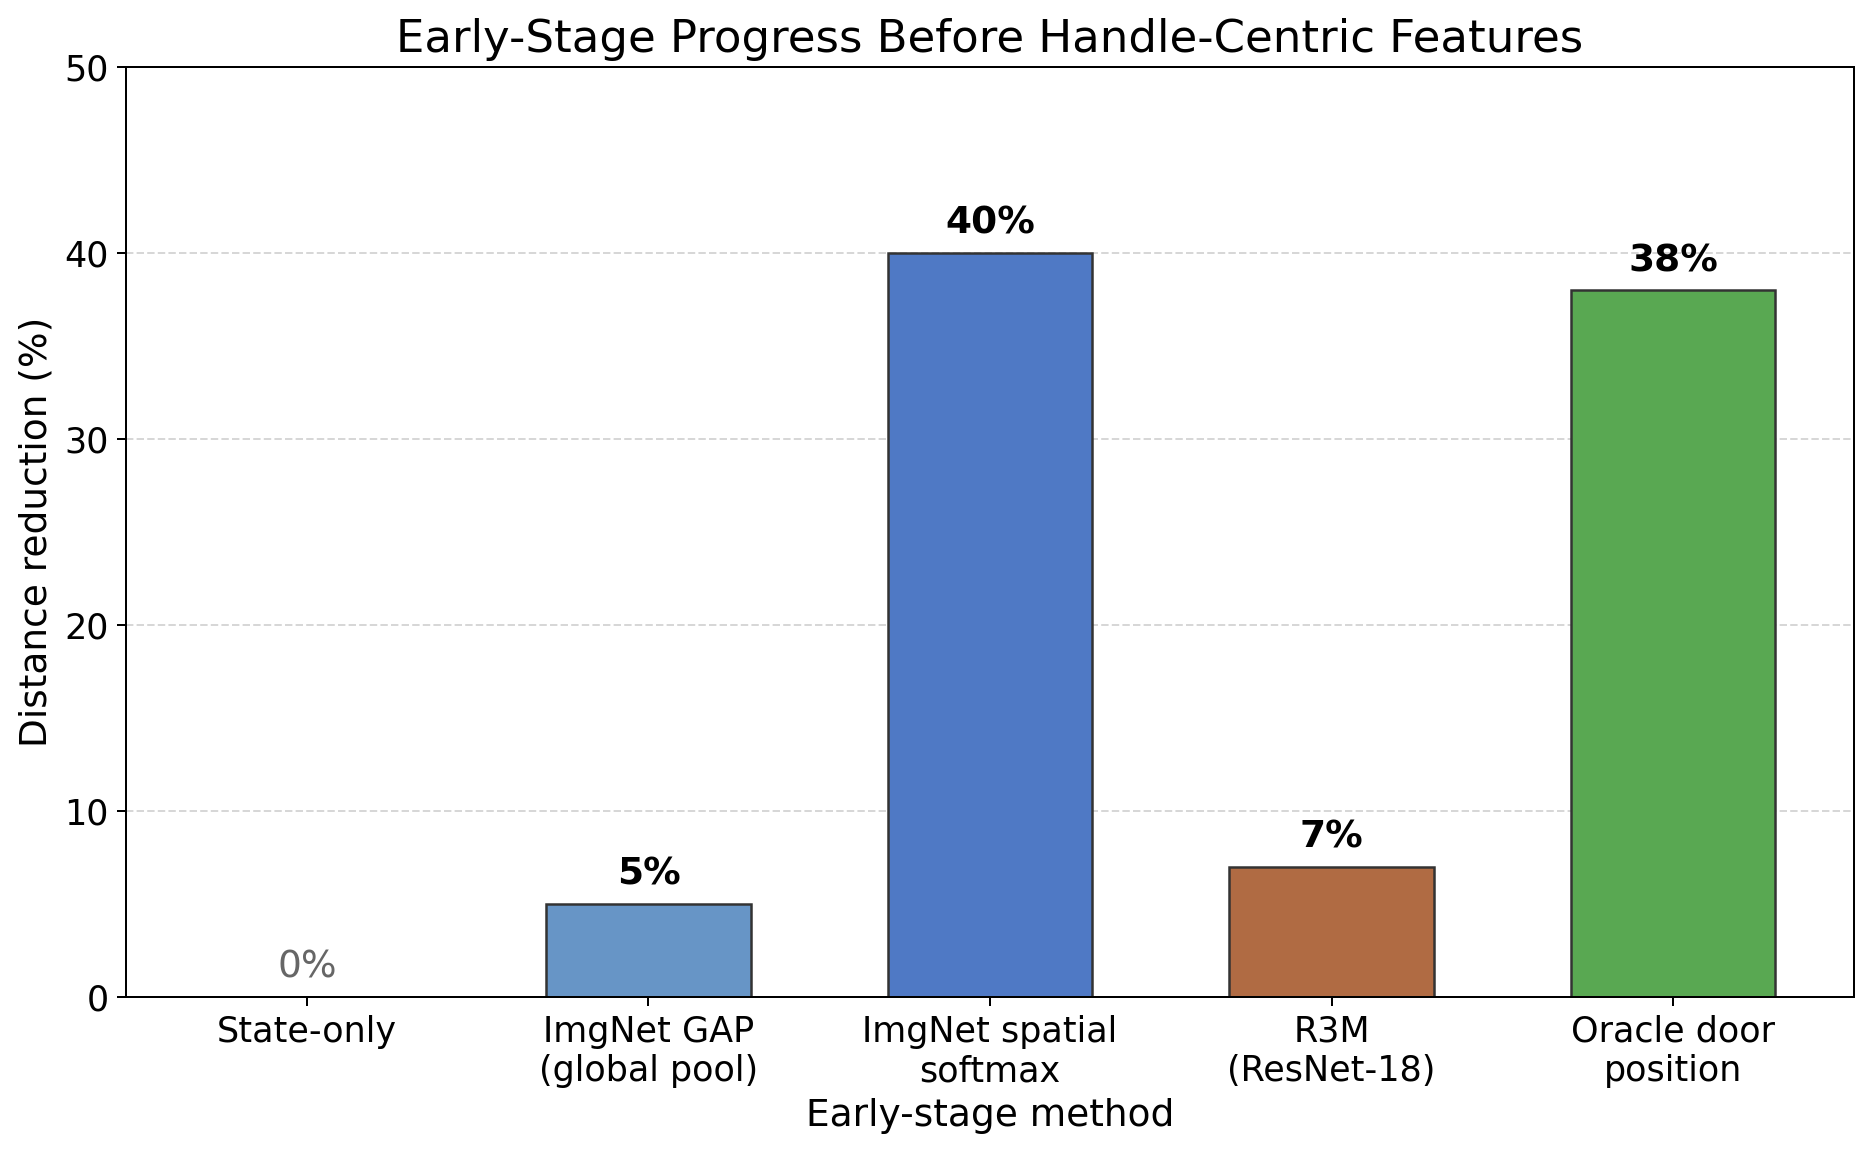
\includegraphics[width=\columnwidth]{assets/early_stage_progress.png}
\caption{Early-stage progress before handle-centric features. Spatially structured visual features improved approach quality relative to state-only or global-pooled baselines, and oracle door geometry provided the strongest pre-handle reduction in target distance.}
\label{fig:early-stage-progress}
\end{figure}

\subsection{Stage 3: BC vs. Diffusion in the 107-Demo Regime}
Once we had stronger geometric features, we compared BC and diffusion directly. In our matched U-Net comparison, BC delivered stronger low-data task performance and trained faster than diffusion. Figure~\ref{fig:bc-vs-diffusion-regimes} shows the broader pattern across data regimes: BC led in the 107-demo setting (44\% vs.\ 10\%), while diffusion improved more with additional data and eventually surpassed BC at 607 demos. In the low-data regime, diffusion's extra expressiveness did not pay off; BC made more efficient use of the small dataset.

\begin{figure}[t]
\centering
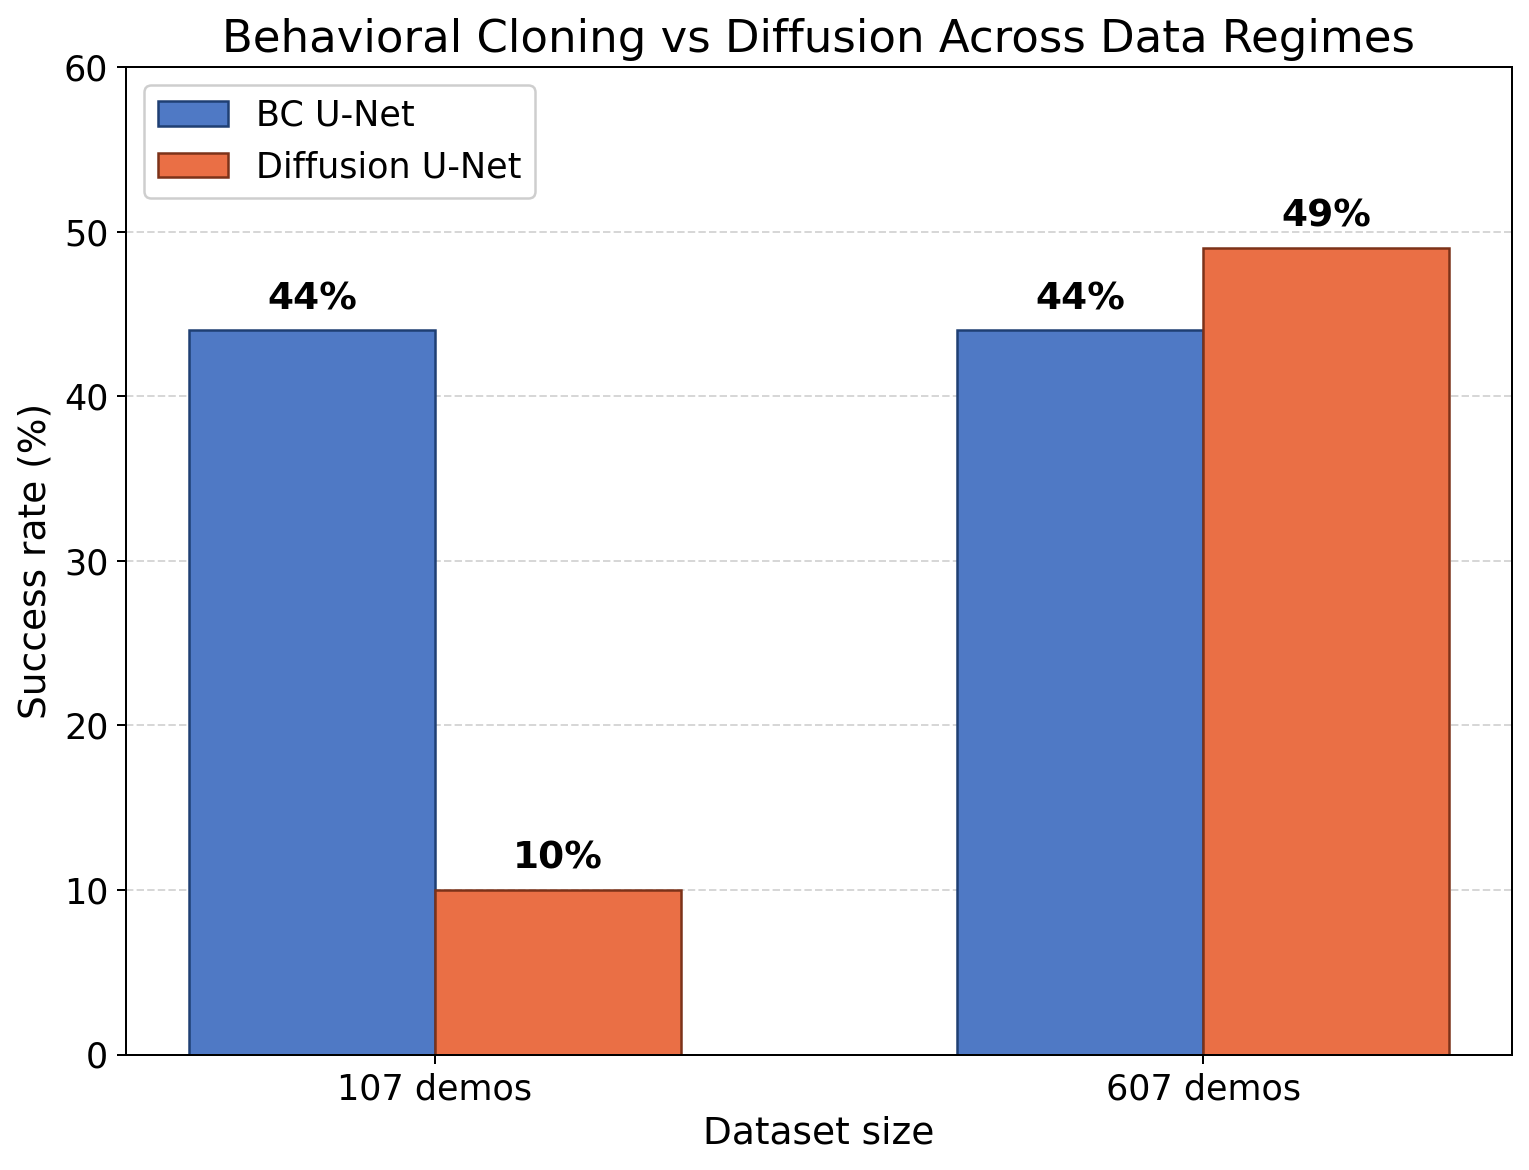
\includegraphics[width=\columnwidth]{assets/bc_vs_diffusion.png}
\caption{Behavioral cloning versus diffusion U-Net across data regimes. BC was stronger in the low-data 107-demo setting, while diffusion benefited more from scaling and achieved the best overall result after expanding to 607 demonstrations.}
\label{fig:bc-vs-diffusion-regimes}
\end{figure}

\subsection{Stage 4: Handle-Centric Features}
The key representation breakthrough was the transition from door-centric to handle-centric state. This change aligned the policy with the true target of the task and yielded a major increase in both distance reduction and success. The reason is simple: the door centroid is not the manipulation target, but the handle is. Once the observation was aligned with the point the robot actually needed to reach and pull, successful interaction became much more attainable.

\begin{table}[H]
\centering
\caption{Representative progression of state representations.}
\footnotesize
\setlength{\tabcolsep}{3pt}
\begin{tabular}{@{}>{\raggedright\arraybackslash}p{0.25\columnwidth}c>{\raggedright\arraybackslash}p{0.22\columnwidth}>{\raggedright\arraybackslash}p{0.26\columnwidth}@{}}
\toprule
Feature Set & Dim & \shortstack{Best\\Result} & Interpretation \\
\midrule
Proprio only & 16 & 0\% success & No cabinet-location signal \\
Door-position oracle & 19 & 5\% success & First nonzero success \\
Full handle-relative transformer state & 44 & 5--10\% success & Enabled handle-aware grasp attempts \\
F3 / final pretrain BC U-Net state & 22 & 44\% success (44/100) & Best pretrain-only result \\
\bottomrule
\end{tabular}
\end{table}

\subsection{Best Pretrain-Only Result}
\begin{table}[H]
\centering
\caption{Best pretrain-only result.}
\footnotesize
\setlength{\tabcolsep}{3pt}
\begin{tabular}{@{}>{\raggedright\arraybackslash}p{0.28\columnwidth}>{\raggedright\arraybackslash}p{0.13\columnwidth}cc>{\raggedright\arraybackslash}p{0.24\columnwidth}@{}}
\toprule
Model & Data & Episodes & Success & Criterion \\
\midrule
BC U-Net (handle-aware) & 107 demos & 100 & 44\% & One door open, hinge angle $> 0.3$ rad \\
\bottomrule
\end{tabular}
\end{table}

Even this strongest pretrain-only model exhibited recognizable failure modes. Some rollouts failed to reach the correct target region, while others approached the handle closely but failed to convert that approach into a stable grasp-and-pull interaction. This suggests that by this stage the main limitation was no longer coarse localization, but fine manipulation quality and gripper execution.

\subsection{Best Overall Result After Data Scaling}
When we expanded to 607 demonstrations, diffusion improved dramatically and finally surpassed BC. This suggests that diffusion had not failed fundamentally in earlier stages; it had simply been more data-hungry, and the larger dataset was enough for its extra modeling capacity to become useful.

\begin{table}[H]
\centering
\caption{Final comparison after data scaling.}
\footnotesize
\setlength{\tabcolsep}{3pt}
\begin{tabular}{@{}>{\raggedright\arraybackslash}p{0.22\columnwidth}>{\raggedright\arraybackslash}p{0.14\columnwidth}c>{\raggedright\arraybackslash}p{0.29\columnwidth}@{}}
\toprule
Model & Data & Success & Notes \\
\midrule
BC U-Net & 607 demos & 44\% & Saturated relative to the low-data result \\
Diffusion U-Net (uniform mix) & 607 demos & 48\% & Improved once more data was available \\
Diffusion U-Net (curriculum mix) & 607 demos & 49\% & Best overall reported result \\
\bottomrule
\end{tabular}
\end{table}

Across these stages, the clearest overall pattern was that representation mattered more than architecture in the early regime. Handle-relative geometry was the most useful signal, BC was the strongest low-data baseline, and diffusion became advantageous only after sufficient data scaling.

\section{Limitations}
Our project has several limitations. The strongest results relied on oracle handle-derived features rather than fully learned perception. Success rates remained far from perfect, especially for consistent grasp-and-pull behavior. Some reported comparisons depend on the specific evaluation criterion used for cabinet opening, and all experiments were conducted in simulation.

\section{Future Work}
Promising future directions include replacing oracle handle features with learned visual localization, improving gripper modeling or contact-aware action heads, incorporating interactive correction or DAgger-style data aggregation, exploring reinforcement learning fine-tuning after imitation, and further scaling diffusion training with larger datasets.

\section{Conclusion}
We studied cabinet-opening imitation learning in RoboCasa through a progression of models, features, and dataset scales. The project showed that state-only policies fail because they lack object information, oracle door features provide the first successful behaviors, and handle-relative features are the true representational breakthrough. In the low-data 107-demo regime, BC U-Net with handle-aware state is the strongest practical method, achieving 44\% success over 100 episodes. After scaling to 607 demonstrations, diffusion U-Net overtakes BC and reaches the best overall performance. The broader lesson is that success in robotic imitation learning depends not just on policy class, but on matching the representation and model complexity to the available data.

\section*{Team Contributions}
\begin{itemize}[leftmargin=1.5em]
    \item \textbf{Noah Cylich:} built the main diffusion-policy and handle-aware experimentation code, including the core \texttt{diffusion\_policy} package, the large ablation and BC-versus-diffusion scripts, the \texttt{bc\_handle.py} handle-relative pipeline, and the running experiment log in \texttt{CURRENT\_RESULTS.md}.
    \item \textbf{Satyajit Kumar:} integrated the preprocessing and dataset-preparation pipeline into the main repo, including oracle replay extraction and validation scripts (\texttt{generate\_door\_positions.py}, \texttt{preprocess\_all\_states.py}, \texttt{prepare\_dataset.py}, \texttt{validate\_best.py}), fixed evaluation logic, and assembled the final project website and media assets.
\end{itemize}

\bibliographystyle{IEEEtran}
\begin{thebibliography}{99}

\bibitem{robocasa}
RoboCasa benchmark website and paper repository. \url{https://robocasa.ai/}.

\bibitem{diffusion_policy}
Cheng Chi, Zhenjia Xu, Sanja Fidler, and other collaborators, ``Diffusion Policy: Visuomotor Policy Learning via Action Diffusion,'' 2023. \url{https://diffusion-policy.cs.columbia.edu/}.

\bibitem{bc}
Stephane Ross, Geoffrey Gordon, and J. Andrew Bagnell, ``A Reduction of Imitation Learning and Structured Prediction to No-Regret Online Learning,'' 2011. \url{https://arxiv.org/abs/1011.0686}.

\end{thebibliography}

\end{document}
